%%%%%%%%%%%%%%%%%%%%%%%%%%%%%%%%%%%%%%%%%%%%%%%
%
% Template per Elaborato di Laurea
% DISI - Dipartimento di Ingegneria e Scienza dell’Informazione
%
% update 2015-09-10
%
% Per la generazione corretta del 
% pdflatex nome_file.tex
% bibtex nome_file.aux
% pdflatex nome_file.tex
% pdflatex nome_file.tex
%
%%%%%%%%%%%%%%%%%%%%%%%%%%%%%%%%%%%%%%%%%%%%%%%

% formato FRONTE RETRO
\documentclass[epsfig,a4paper,11pt,titlepage,twoside,openany]{book}
\usepackage{epsfig}
\usepackage{plain}
\usepackage{setspace}
\usepackage{amsmath}
\usepackage{amssymb}
\usepackage{url}
\usepackage{subfigure}
\usepackage{multirow}
\usepackage{array}
\usepackage{rotating}
\usepackage{algorithm}
\usepackage[noend]{algpseudocode}
\usepackage{fancyvrb}
\usepackage[paperheight=29.7cm,paperwidth=21cm,outer=1.5cm,inner=2.5cm,top=2cm,bottom=2cm]{geometry} % per definizione layout
\usepackage{titlesec} % per formato custom dei titoli dei capitoli
\usepackage{tikz}
\usetikzlibrary{positioning}

%%%%%%%%%%%%%%
% supporto lettere accentate
%
%\usepackage[latin1]{inputenc} % per Windows;
%\usepackage[utf8x]{inputenc} % per Linux (richiede il pacchetto unicode);
\usepackage[applemac]{inputenc} % per Mac.

\singlespacing

\usepackage[english]{babel}

\newcommand\MyBox[2]{
  \fbox{\lower0.75cm
    \vbox to 1.7cm{\vfil
      \hbox to 1.7cm{\hfil\parbox{1.4cm}{\centerline{#1}}\hfil}
      \vfil}%
  }%
}

\begin{document}

  % nessuna numerazione
  \pagenumbering{gobble} 
  \pagestyle{plain}

\thispagestyle{empty}

\begin{center}
  \begin{figure}[h!]
    \centerline{
\psfig{file=logo_unitn_black_center.eps,width=0.6\textwidth}}
  \end{figure}

  \vspace{2 cm} 

  \LARGE{Dipartimento di Ingegneria e Scienza dell’Informazione\\}

  \vspace{1 cm} 
  \Large{Corso di Laurea in\\
    ...
    %Informatica
    %Ingegneria dell'Informazione e delle Comunicazioni
    %Ingegneria dell'Informazione e Organizzazione d'Impresa
    %Ingegneria Elettronica e delle Telecomunicazioni
  }

  \vspace{2 cm} 
  \Large\textsc{Elaborato finale\\} 
  \vspace{1 cm} 
  \Huge\textsc{Titolo\\}
  \Large{\it{Sottotitolo (alcune volte lungo - opzionale)}}


  \vspace{2 cm} 
  \begin{tabular*}{\textwidth}{ c @{\extracolsep{\fill}} c }
  \Large{Supervisore} & \Large{Laureando}\\
  \Large{......}& \Large{......}\\
  \end{tabular*}

  \vspace{2 cm} 

  \Large{Anno accademico .../...}
  
\end{center}



  \clearpage
 
%%%%%%%%%%%%%%%%%%%%%%%%%%%%%%%%%%%%%%%%%%%%%%%%%%%%%%%%%%%%%%%%%%%%%%%%%%
%%%%%%%%%%%%%%%%%%%%%%%%%%%%%%%%%%%%%%%%%%%%%%%%%%%%%%%%%%%%%%%%%%%%%%%%%%
%% Nota
%%%%%%%%%%%%%%%%%%%%%%%%%%%%%%%%%%%%%%%%%%%%%%%%%%%%%%%%%%%%%%%%%%%%%%%%%%
%% Sezione Ringraziamenti opzionale
%%%%%%%%%%%%%%%%%%%%%%%%%%%%%%%%%%%%%%%%%%%%%%%%%%%%%%%%%%%%%%%%%%%%%%%%%%
%%%%%%%%%%%%%%%%%%%%%%%%%%%%%%%%%%%%%%%%%%%%%%%%%%%%%%%%%%%%%%%%%%%%%%%%%%
  \thispagestyle{empty}

\begin{center}
  {\bf \Huge Acknowledgments}
\end{center}

\vspace{4cm}


\emph{
I dedicate my bachelor's thesis to my beloved grandmother. I want to thank all the people that have supported me during this three years, especially my family, my aunt Tiziana and my girlfriend Arianna. A special thanks goes to those that made possible this thesis: my university supervisor Alberto Montresor; Daniele Miorandi, who guided me every day during the internship and the drafting of the thesis; all the U-Hopper family, to gave me the chance to work in such a fantastic environment. In alphabetical order: Carlo, Christian, Daniele, Diego, Federico, Mozhdeh and Rossana.
}

  \clearpage
  \pagestyle{plain} % nessuna intestazione e pie pagina con numero al centro

  
  % inizio numerazione pagine in numeri arabi
  \mainmatter

%%%%%%%%%%%%%%%%%%%%%%%%%%%%%%%%%%%%%%%%%%%%%%%%%%%%%%%%%%%%%%%%%%%%%%%%%%
%%%%%%%%%%%%%%%%%%%%%%%%%%%%%%%%%%%%%%%%%%%%%%%%%%%%%%%%%%%%%%%%%%%%%%%%%%
%% Nota
%%%%%%%%%%%%%%%%%%%%%%%%%%%%%%%%%%%%%%%%%%%%%%%%%%%%%%%%%%%%%%%%%%%%%%%%%%
%% Si ricorda che il numero massimo di facciate e' 30.
%% Nel conteggio delle facciate sono incluse 
%%   indice
%%   sommario
%%   capitoli
%% Dal conteggio delle facciate sono escluse
%%   frontespizio
%%   ringraziamenti
%%   allegati    
%%%%%%%%%%%%%%%%%%%%%%%%%%%%%%%%%%%%%%%%%%%%%%%%%%%%%%%%%%%%%%%%%%%%%%%%%%
%%%%%%%%%%%%%%%%%%%%%%%%%%%%%%%%%%%%%%%%%%%%%%%%%%%%%%%%%%%%%%%%%%%%%%%%%%

    % indice
    \tableofcontents
    \clearpage
    
    
          
    % gruppo per definizone di successione capitoli senza interruzione di pagina
    \begingroup
      % nessuna interruzione di pagina tra capitoli
      % ridefinizione dei comandi di clear page
      \renewcommand{\cleardoublepage}{} 
      \renewcommand{\clearpage}{} 
      % redefinizione del formato del titolo del capitolo
      % da formato
      %   Capitolo X
      %   Titolo capitolo
      % a formato
      %   X   Titolo capitolo
      
      \titleformat{\chapter}
        {\normalfont\Huge\bfseries}{\thechapter}{1em}{}
        
      \titlespacing*{\chapter}{0pt}{0.59in}{0.02in}
      \titlespacing*{\section}{0pt}{0.20in}{0.02in}
      \titlespacing*{\subsection}{0pt}{0.10in}{0.02in}
      
      % sommario
      \chapter*{Summary} % senza numerazione
\label{summary}
\addcontentsline{toc}{chapter}{Summary} % da aggiungere comunque all'indice
Everyone's life is full of events, some of these are daily routines, some are minor and not too much attention is given to them, and some others are real milestones. The latter ones are what will be called \emph{Life Events}: according to Cambridge Dictionary\footnote{\url{dictionary.cambridge.org}}, they are \textit{"a very important event in someone's life, such as marriage, the birth of a child, or the death of a family member"}. These kind of events are quite rare in a lifetime, and they may bring with them a big charge of stress, and big changes for those who live it. Furthermore, they don't last only for the day they happen, but there is a medium or long period that is influenced by the event: for example, a pregnancy lasts for 40 weeks, or a wedding is usually organized in several months; but also a negative life event, like the death of someone dear, causes bad feelings for a period more or less long for those who live it. The Holmes and Rahe stress scale \cite{holmes1967social} puts in relation several life events for the load of stress they cause: on a scale from 0 to 100, the most stressful event for an adult is the death of a spouse, that scores 100, but also positive events are part of this list, such as marriage, with the score of 50, and a pregnancy, with 40. In addition, a life event can be followed by another one life event: for example in Italy, the 80\% of births occur within a marriage in 2012\footnote{\url{www.istat.it/it/files//2015/02/Avere_Figli.pdf}}.

Therefore, a life event it's a signal of many factors in who lives it. If it is detected in time, it can be a great opportunity for many entities, such as banks, insurance companies and other kinds of ad-hoc marketing campaigns. The life events have a deep effect on the individual's spending habits and purchase patterns. According to the results\footnote{\url{travelbehaviour.files.wordpress.com/2014/06/lttb_carownbriefingnote_16-june.pdf}} of a study made by the University of the West of England about the relationship between life events and Travel behaviour \cite{chatterjee2015facts}, households are more likely to change the number of cars at the time of life events: the "\textit{Birth of a child increases likelihood of a non-car owning household acquiring a car and increases likelihood of a two-car owning household relinquishing a car. This suggests households seek a one car solution when having children}".

Nowadays one of the most common way to make announcements or to share something about private life is via \emph{social networks}. A social network is a web application that allows users to create their own network of friends and relationships, sharing their news feed and reading that of others. The 
catchment area of these services has grown exponentially by size in the last few years: for example Facebook has more than 2.2 billion monthly active users as of January 2018. For the huge flows of information daily shared on these platforms they have been compared with the industrial media, such as newspapers and televisions, being called also \emph{social media}.

In this thesis is presented a system that is able to detect a life event into someone's social timeline, using a hybrid technique to perform its scopes: a machine learning based method to make post classification, and a model based approach to analyze the timeline. The system is designed to work with many social networks, and to inspect both texts and photos. It doesn't use any text or picture analysis technique, but a method based on the Wikipedia entities is used to understand the content and the meaning of photos and texts.

In addition to that, a new freely available dataset about life event classification on Twitter has been release, which counts more than 5000 samples written by 45 users, and which is very unbalance, like a real social timeline.

In conclusion, this thesis work makes a move forward to the actual state of the art about life event detection on social media: nowadays the literature doesn't offer any kind of solution that analyzes a user's timeline for this purpose. The system that will be presented takes care of every step needed to do that: providing the ID of the user to analyze on a given social network, and a life event to search for, it deals with content downloads, content classification and user's timeline analysis, returning a list of time ranges, one for each identified event.


%%%%%%%%%%%%%%%%%%%%%%%%%%%%%%%%%%%%%%%%%%%%%%%%%%%%%%%%%%%%%%%%%%%%%%%%%%
%%%%%%%%%%%%%%%%%%%%%%%%%%%%%%%%%%%%%%%%%%%%%%%%%%%%%%%%%%%%%%%%%%%%%%%%%%
%% Nota
%%%%%%%%%%%%%%%%%%%%%%%%%%%%%%%%%%%%%%%%%%%%%%%%%%%%%%%%%%%%%%%%%%%%%%%%%%
%% Sommario e' un breve riassunto del lavoro svolto dove si descrive 
%% l’obiettivo, l’oggetto della tesi, le metodologie e 
%% le tecniche usate, i dati elaborati e la spiegazione delle conclusioni 
%% alle quali siete arrivati.
%% Il sommario dell’elaborato consiste al massimo di 3 pagine e deve contenere le seguenti informazioni: 
%%   contesto e motivazioni
%%   breve riassunto del problema affrontato
%%   tecniche utilizzate e/o sviluppate
%%   risultati raggiunti, sottolineando il contributo personale del laureando/a
%%%%%%%%%%%%%%%%%%%%%%%%%%%%%%%%%%%%%%%%%%%%%%%%%%%%%%%%%%%%%%%%%%%%%%%%%%
%%%%%%%%%%%%%%%%%%%%%%%%%%%%%%%%%%%%%%%%%%%%%%%%%%%%%%%%%%%%%%%%%%%%%%%%%%      
      
      %%%%%%%%%%%%%%%%%%%%%%%%%%%%%%%%
      % lista dei capitoli
      %
      % \input oppure \include
      %
      \chapter{Introduction}
\label{cha:intro}

This thesis work was developed during a 4 month internship at U-Hopper\footnote{\url{u-hopper.com}}, with which I was able to combine a work experience in a company with the writing of the bachelor's thesis. U-Hopper is a research-intensive deep-tech SME, headquartered in Trento, providing big data-enabled solutions and technologies for the government, retail and manufacturing sectors. U-Hopper has received numerous awards for its innovative solutions, including, among the others, the Lamarck prize (2013), a EC Seal of Excellence (2015), the Innov@Retail prize (2016) and a nomination for the 2017 EC Innovation Radar Awards. Life event detection can be a significant business for the company, because it is already into the user profiling world, with a product called Tapoi\footnote{\url{www.tapoi.me}}, but above all because detect a life event into someone's life can bring many opportunity with banks, insurances, estate agents and many other businesses, which are constantly looking for such a meaningful information like a life event can be.

A life event is a kind of event that is rare into someone's life, which brings with it many actions and many consequences. It is a life changing milestone for everyone, which implies new habits and new needs for who lives it: thinking about the birth of a child, a family may need a bigger car or a bigger house, a life insurance for the baby, or even a new job position with different working time for a parent. For these reasons, many entities can use a life event discovery to create ad-hoc advertising campaign. 

The identification of a life event into social media contents is a \emph{machine learning} problem, and to be more precise, a classification one. Machine learning is a field of computer science which deals with allowing a computer system to "\textit{learn with data, without being explicitly programmed}" \cite{samuel1959some}. It can be applied in many contexts, such as taking decisions, or make optimizations, forecasts and predictions. Nowadays a human being faces itself with machine learning in everyday life: home assistants, security surveillance, music and shopping suggestions, customer services are strongly powered by artificial intelligence. These services relies on data to learn how to work as good as possible: they are trained with samples of data similar to what they expect to receive by their users: the more accurate, exhaustive and in large quantities they are, the better the system learns. Therefore, data have a very central role in machine learning problems.

A classification task has the goal of assigning a belonging class to a given object. The input is composed by a tuple of \emph{features} that characterize the object, usually made by numbers, and the output is a categorical variable, such as a "yes/no" label. In other words, it can be seen as a mathematical function, that maps a vector $ \boldsymbol{x} \in \mathbb{R}^n $ to an answer $ y \in C $
\begin{gather*}
\begin{split}
f & \colon \mathbb{R}^n \to C \\
f & \colon \boldsymbol{x} \mapsto y
\end{split}
\end{gather*}
where $C$ is a set of possible categories. A famous educational example of this kind of problem is the Iris flower classification\footnote{\url{en.wikipedia.org/wiki/Iris_flower_data_set}}, where the input $ \boldsymbol{x} $ is composed by the sepal and petal widths and lengths in cm of the flower, and $C = \{\text{\texttt{Iris setosa}, \texttt{Iris virginica}, \texttt{Iris versicolor}}\}$. For each sample composed by 4 measures the belonging class is predicted.

The background of live event identification on social media consists in a huge stream of documents, called \emph{posts}, each one written by a specific user and containing text, images, external links and other attachments, with a date of publication. Every user can share, comment or like someone else's post. A \emph{timeline} is the list of posts written by a single user, sorted by decreasing date of publication. These data are accessible through the Web (in some cases the author's authorization is necessary to get them) and contain many information. There is an endless number of works that use social media data for various purposes, and in this case they are used to detect events.

\section{Research objectives}
Life event detection on social media is still an open problem; in fact, such a commercial solution to be integrated into a social system of some commercial, banking or insurance entity does not exist, not even an accademic pubblication that goes beyond a classification problem. Therefore, the reseach question is the following: \emph{is it feasible to detect the occurrence of life events based on social media user activities?}

The goal of this thesis is to find a way to understand whether a person has lived a life event, or if she is about to live it, observing her activities on social media. Nowadays, social media are widely used all over the world: according to the Global Digital 2018 report\footnote{\url{wearesocial.com/it/blog/2018/01/global-digital-report-2018}}, 3.196 billions of people use social media every month, sharing messages, photos and other contents that are also about their private life. They are used to deliver messages of congratulations or support, to search for information from users who have experienced certain situations or to make announcements of news or changes. Consequently, social media are one of the best platform to get reliable information about people in an easy, fast and free way.

The idea is to design a hybrid system that combines a data driven approach to analyze each post, and a model driven solution to inspect a user's timeline, in order to find out whether the user has lived a life event according to what she shared on social media. This work is focused on the detection of two life events, marriages and births of a child.

\section{Detection vs prediction}

A user's timeline is composed by all the posts published from the time she signed up to the social media up to today. From this data is possible to \emph{detect} an event that happened in the past. Event detection is the identification of an event that occurred, into a stream of data, and now it is finished or at most it is still ongoing. Another possibility is to \emph{predict} an event, understanding whether the event can occur in a more or less near future. Event prediction can be done in several ways, for example observing what happen in the user's past, or in timelines of users with similar age, location and preferences, or using some logical model: for example, a married person will likely have a baby in her lifetime.

Of course, the two things have a very different meaning. With event detection is possible to understand what a person lived in the past, what she might searched or needed at the time of the event, and which are her usual needs: for example, if it is known that a user had a child, her possible future vehicle will be a family car, or her new house should probably have at least two bedrooms. With event prediction is possible to anticipate some user's choices or needs, giving her some ad-hoc offers and advertising campaign: for example, if it was known that a user would probably have a child in the near future, she would likely look for a new bedroom furniture or a new bigger car.

From the machine learning point of view there is no big differences between event detection and event prediction. In both cases the usual patterns that indicate that the event is about to occur are the same. The only difference is that the detection is based on facts, and so it is possible to say whether the obtained result is correct or not, while prediction is based on suppositions, which are not always verifiable. This thesis is focused on life event detection, so on what the user has lived.

\section{Outline}

This thesis work is organized as follows: in Chapter 2 the state of the art is introduced, explaining what is missing for this purpose and what has to be changed. In addition, the data situation about life event will be shown, unfolding a solution that is different from the standard text classification. In Chapter 3 the design solution is presented, with a particular focus on the logical behind the system and on the used algorithms. Chapter 4 is about the implementation procedure and the performance evaluation of a prototype of the system, and finally, in Chapter 5 some final remarks and observations for future developments are presented.


      \chapter{State of the Art}
\label{cha:soa}

In this chapter the state of the art in dealing with life events on social media will be presented, starting with what the research has done so far to detect them, and explaining also the current situation with data in this field.

Event detection using social networks is a common practice. The literature offers many example of event detection on a global scale based on the analysis of social media contents, such as real-time earthquake identification based on tweets \cite{sakaki2010earthquake}, breaking news discovery in Twitter \cite{jackoway2011identification, phuvipadawat2010breaking}, or big gigs recognition observing what is posted on Flickr \cite{liu2011using}.

Event prediction using social network contents is also pretty common: the most striking example of the last few years are the 2016 american elections. In fact, while many of the official polls made by the most famous american newspapers and televisions had always forecasted Hillary Clinton as winner, social media reactions had been increasingly in favor of the Republicans during the election campaign\footnote{\url{https://techcrunch.com/2016/11/10/social-media-did-a-better-job-at-predicting-trumps-win-than-the-polls}}, and the rest is history. Other cases of event prediction using social media are, for example, movie box-office \cite{asur2010predicting} or Oscar-winner forecasts.

There is much less literature about life-event detection on social media, and it is almost completely focused on post classification. Another important issue about life events is related with data: it's hard to find it, and in a machine learning scenario like this problem data play a key role.

\section{Life event detectors on social media}
\label{sec:socialmediadetectors}
Almost every model proposed by the literature are classifiers that take a textual post as input and give as output a label, indicating whether the text talks about a life event. Each classifier is specialized to a single life event, for example a detector of posts about weddings. Some models are focused on a single post at a time, while few others \cite{cavalin2015multiple, moyanolife} consider also the conversation linked to the main post to understand the content and the importance of the speech. The feature extraction is done mainly in two ways: working with the text itself, using bag-of-words or bag-of-N-grams \cite{cavalinclassification, di2013detecting, li2014major}, or using a semantic analyzer, to obtain sentiment score, formality with which the text is written, entities and topics contained, etc \cite{khobarekar2013detecting}. Both methods are used combined together as well. In addition to that, some models consider also "external" features, like user's features (number of friends, age, location, post frequency, etc.) or post success \cite{dickinson2015identifying}.

All these models have several weaknesses for the purpose of this thesis, and they will be briefly described now. First of all, they are only classifiers that take into consideration a single post at the time labelling it, they don't go further with the information they obtain. Secondly, there is no consideration of the user timeline, of her behavior on social media, and no comparison with other posts published by the same user: in fact data is fetch more or less randomly from the social networks, without any user profiling intent, and consequently each post analyzed is completely disconnected with the other ones. Furthermore, analysing contents in this way there is no perception of how much the event may have lasted, and it is not understandable whether the event was in the past and now it's over, is just passed, it's occurring or it's coming in the near future. Another point worth of noting is that a post related to a life event may not be concerned with the author (e.g. participate to a wedding instead of getting married), or a post classified as about a life event could be a false positive: in both cases the decision to say that this person has lived a life event is based only on a single content, and this is a result of not consider the user's timeline. Thirdly, only text contents are considered: however, according to Mark Zuckerberg, CEO and founder of Facebook, "\textit{Most of the content 10 years ago was text, and then photos, and now it's quickly becoming videos}"\footnote{\url{https://www.fastcompany.com/3057024/mark-zuckerberg-soon-the-majority-of-content-we-consume-will-be-video}}. Not only are posts composed by more than only text, but many of them have no text at all. Furthermore, the meaning of an image or a video can give a strong clue to understand what the post is about: for example, an image containing a pink ribbon can easily be interpreted as a female baby announcement, without even look at the text. Last but not least, every model cited above uses Twitter contents only: this platform allows to share texts with at most 280 characters (until late 2017 the limit was 140) and it's used more for business purposes rather than personal life sharing. On the other hand, most of the contents on this social network are free to access and to obtain, without explicit user authorization.

\subsection{A step further}
The literature offers a model that goes a step further of those highlighted above: the work made by Cavalin, Gatti, Pinharez for the \textit{IBM InfoSphere BigInsights} platform \cite{cavalin2014towards}, starting from life event classification on a sample of tweets, it performs a user entity matching on an existing database of clients, aimed to decide which is the best approach to offer them some services or some products. Once a user that texts about a life event is identified, her information are used to match her into a database of clients.

In common with our model there is a big move forward from a simple classifier, but with an important difference: it solves the reverse problem of ours. Its goal is to get a list of users that posted about a life event in a given time window, while ours is to understand if a user has posted about a life event and in which time period. In this paper a wide range of posts written by many authors is taken to analyse the presence of a life event, not considering user's timeline at all, while our model is focused on a single user analysis. This brings all the problems highlighted above in the previous section. Furthermore, also this model is  concentrated only on Twitter contents.

\section{Other interesting methods}
In addition to the previous models, the literature offers several works that are methodologically interesting. They will be briefly described now.

As already mentioned, life event detection is a branch of event identification. The core of the business is therefore the identification of events from a stream of time-stamped documents coming from social networks. In concrete, the job made by Vavliakis, Symeonidis and Mitkas \cite{vavliakis2013event} organizes documents from various sources according to the event they describe, assigning to the event an importance, while the one made by CC Chen, MC Chen and MS Chen \cite{chen2009adaptive} tracks how much activity is related to an event from a global stream of documents. However, also these two models work on global scale, not analyzing a specific user, and they have an implicit issue: they consider the importance of the event based on the \textit{noise} the event brings with him. The more people talk about an event, the more important it is. Therefore every global event, such as The Olympics, will be classified as much more important than a wedding or a birth of a child.

Another interesting study is the one proposed by Li, Ritter and Jurafsky \cite{li2014inferring}, a model-driven system to infer user's attitudes or preferences reasoning over user's attributes and social network graphs. It builds, for every person taken into analysis, a series of predicates for her attributes (location, gender, education), relationships (married, friends) and preferences (what she likes/dislikes), which can be used to detect important events on her timeline or in friends/relatives social profiles. This work is interesting beacuse is the only one that is not completely driven by data and machine learning, but it offers a logical model, and also it combines multiple social networks (Twitter and Google+). On the other hand, of course, this model is not designed to deal with life events.

A last interesting study is about topic sentiment analysis using the hashtag graph in Twitter \cite{wang2011topic}. It demonstrates that hashtags offer additional information to texts, classifying tweets and users in categories: the use of a specific hashtag may be connected with a specific life event. This kind of study, however, has more sense on global scale analysis, like searching for users who show interest in a specific topic: it may be not so useful in a context of life event detection, which is concentrated on a single-user analysis.


\section{The dataset problem}
\label{sec:dataset}
One of the biggest issue in dealing with life events is the lack of data. For an artificial intelligence powered solution a great amount of data is needed, to train a machine learning system and to evaluate it. Furthermore, very few benchmarks exist, so it's hard to understand which is a good result to reach and what are the minimum expectations.

Many users don't share with the world what happens to them in their private life, in fact most of the posts on social networks are not about users' personal life. There is also a strong subjectivity in sharing a life changing event: every user has her way to announce a personal news and it's hard to find a pattern that identifies a life event announcement. For these reasons is not easy to build a dataset big and reliable enough to train the system as good as possible. Furthermore, among the papers cited above, only one \cite{dickinson2015identifying} published the dataset build for the experiment\footnote{\url{http://reellives.net/rl-data/uploads/2015/06/a692044.csv}}.

The literature presents two different ways to fetch and label the data. Some authors prefer to fetch only contents that contain specific keywords (such as "\textit{engagement}" for marriage) \cite{dickinson2015identifying, khobarekar2013detecting}, labelling each content \textit{by hand} as about or not to the life event itself; some other search for contents randomly, labelling it in a more automatic way, considering a text related to the life event if it contains at least one keyword \cite{choudhury2014personal, di2013detecting, moyanolife}. The first method requires a bigger effort than the second one, because data is selected before the download, and once downloaded is analyzed by a human, who assigns to each post a relation with a life event. On the other hand, bigger work leads to better precision: a human classification is not based on the content only, but also on the meaning of the text. Of course this approach for huge datasets (those used into the cited papers with \textit{automatic} labelling space from tens of thousands to millions of samples) is not recommended. 

In case more than one life event is taken into consideration, this kind of classification becomes a multi-label classification. For example, if marriage and birth of a child are considered, a tweet that speaks about a wedding will have the \textit{marriage} label setted to \texttt{true}, and the \textit{having children} label setted to \texttt{false}. According to \cite{cavalinclassification} and to Wikipedia\footnote{\url{https://en.wikipedia.org/wiki/Multi-label_classification}}, the easiest way to perform this type of classification is doing a set of binary classification: to do that, a dataset for each life event is necessary. Another problem is represented by how many languages the classifier wants to support: for each of them is necessary a satisfying number of samples, to allow the classifier to learn any patterns or idioms related to each language. In conclusion, if the methodologies exposed by these works were followed, a dataset for each life event and for each language would be necessary. For example, a system that classifies posts about marriage and birth of a child written in english and italian, would need 4 datasets: marriage-english, marriage-italian, child-english and child-italian.

The solution chosen to overcome the language issue was inspired by the user profiling software made by U-Hopper, called Tapoi\footnote{\url{http://www.tapoi.me}}, which works with Wikipedia\footnote{\url{https://www.wikipedia.org/}} to understand what a user has talked about in her social profiles \cite{torrero2018wikipedia}. The idea is to use Wikipedia articles to classify words, topics and concepts inside a phrase: each post will contain a set of articles, called \textit{entities}, and categories, called \textit{topics}, which will be the features for the classification. Instead of using the classical bag-of-words with texts, a \textit{bag-of-Wikipedia-entities} will be applied. The procedure is the following: firstly, a dataset in a given language has to be provided; secondly, each post of the dataset has to be analyzed by some semantic analyzer, to extract Wikipedia entities and concepts; thirdly, a machine learning classifier is trained using Wikipedia entities and concepts as feature. Once the classifier is ready, the procedure of analyzing posts with a semantic analyzer must be done with every post to classify. In case a post is written in a language that is not the one of the training set, its entities and concepts have to be translated into those belonging to the Wikipedia version of the training set language.

In addition to that, is possible to use Wikipedia entities not only in texts, but also with images. In fact, there are several image analyzers that are able to find out entities into pictures. In this way is not necessary to create a training set also for images, but it is enough to use the same dataset of texts.


      \chapter{System design}
\label{cha:design}

\begin{figure}
\centering
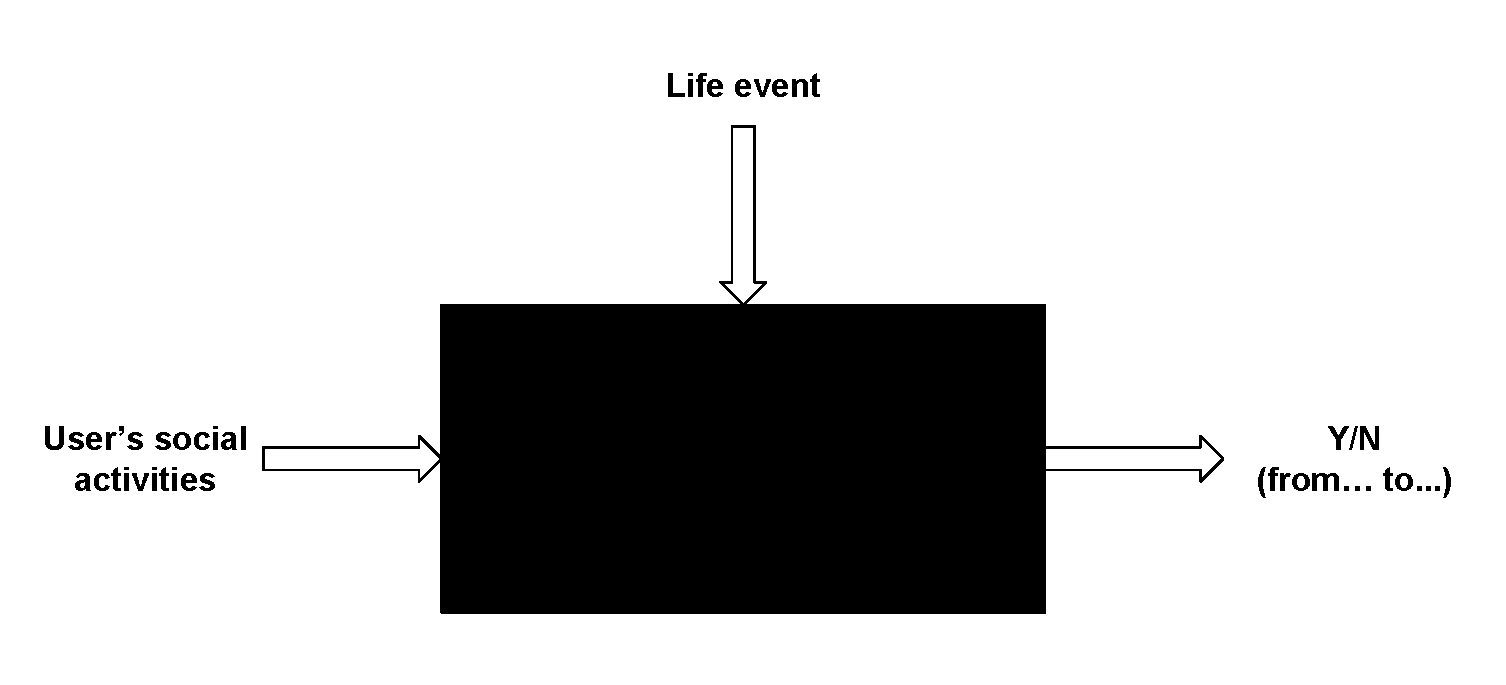
\includegraphics[width=%
0.95\textwidth]{img/bb}
\caption{A black box view of the problem.}
\label{fig:bb}
\end{figure}

In this chapter the design process will be presented, starting from the requirements and the description of the working logic. After that, a more schematic view will be provided, explaining how the system is designed and how the components work and communicate each other. At the end, the algorithms used to compute the output will be presented and explained.

Seen as a black-box (in figure~\ref{fig:bb}), the system takes two inputs: all the user's activities in the social networks she is registered in, and a life event to search for, and it returns as output a yes/no answer to the question "\textit{has this user lived this life event?}", with a time reference estimation attached.

\section{Requirements}

The main requirement is that the software solution has to be able to decide whether the user taken into analysis has lived a given life event. The decision has to be taken analyzing her activities on the social networks she is registered in. The time required to perform this computation should not be long, although data come from an online stream of contents.

Other requirements expect to let the addition of a new user to analyze, or to add and remove a social media account to an already existing user.

The set $S$ of life event that can be searched for should be defined a priori, and should be: 
\[
S = \{\text{\texttt{Getting married}}, \text{ \texttt{Having children}}\}
\]

\section{Logical components}
\label{sec:logicdescr}

\begin{figure}[b]
\centering
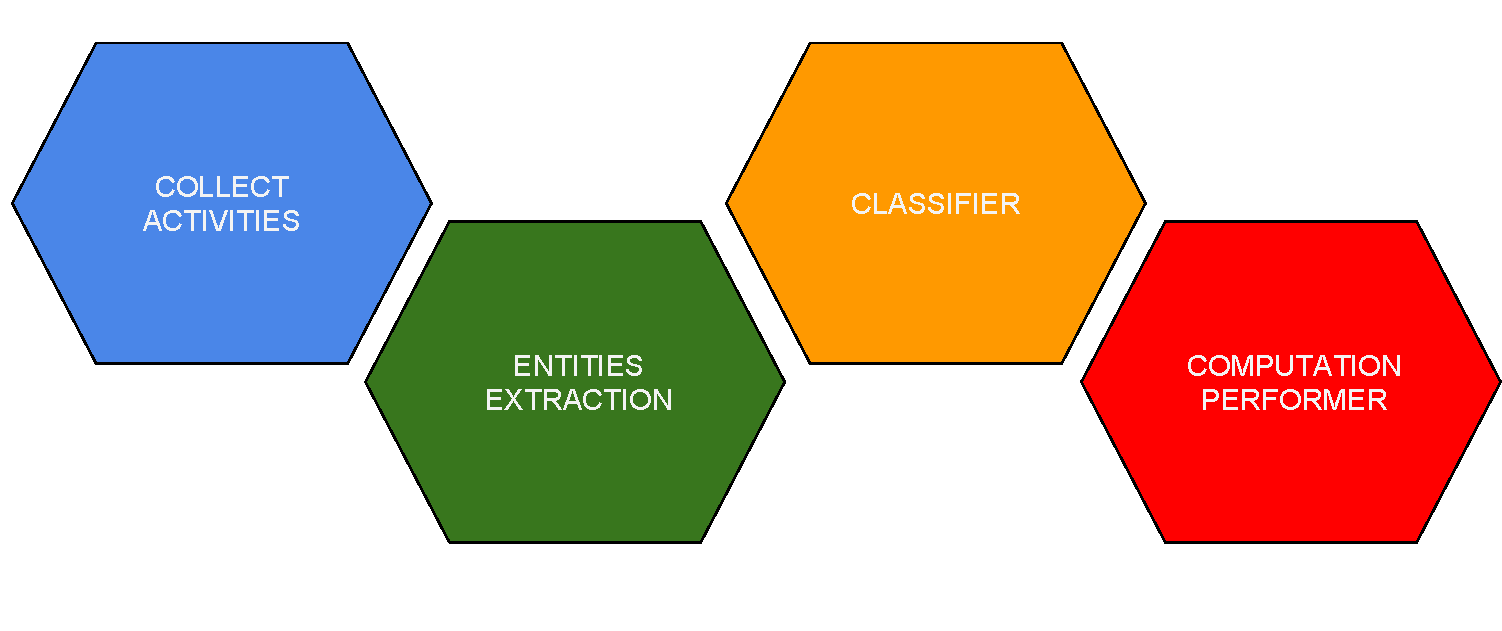
\includegraphics[width=%
0.95\textwidth]{img/Solutiondesign_nutshell}
\caption{The solution design in a nutshell.}
\label{fig:nutshell}
\end{figure}

This section describes the specifications of the logical functionalities of the system. Each functionality is a group of actions whose purpose is to carry out a section of the job required to go from row data - a user identifier - to a piece of information - the answer to the question "Has this person lived a life event?". The steps are the following, as shown in figure~\ref{fig:nutshell}:
\begin{enumerate}
\item Collect activities from social networks.
\item Extract semantic entities from social network contents.
\item Classify each content.
\item Decide whether the user has lived the life event relying on his/her contents.
\end{enumerate}
Each step relies on what the previous steps do: for example, to execute the third one, the first and the second ones must have already been executed at least once. The number of execution required to perform the entire computation from scratch will probably not be the same for each part: in fact, the first two steps are coupled together, and they need to be performed a consistent number of times before fetching an entire user's timeline. Once the whole timeline is downloaded, just a single call for the third and the fourth steps will be needed to complete the computation. In the following subsections the logic of the proposed methodology will be illustrated, providing a textual description of what each component has to do, of the input, the output and the parameters. 

\subsection{Collect activities}
This part has the goal to fetch user's contents on social networks, using the services for developers offered by the official APIs of each social network. The data of interest are some pieces of user's information, such as name, birthday, number of friends/followers, subscription date, her location and language, and of course all her contents: all the posts she wrote, with attachments, external links and the publication date, with also some other useful metadata, such us the number of likes, replies and shares. Some social media, like Twitter, offer a free API plan with some restrictions over time: for example to retrieve user's tweets is possible to make 1500 requests every 15 minutes. In case the limit is reached, this part should suspend itself waiting for a new time slot: for this reason is suggested to run this function in a dedicated thread or process.

As input this functionality needs a series of IDs that identify the user among all the social networks she uses, and for each social platform is necessary to know at which point the data of a given user has been downloaded. In fact, due to the huge amount of data, social network services return a small quantity of data for each request, therefore, after the first request, the point from which start to download data must be specified.

As output, a list with \emph{new} user's post is expected. In case it's the first time that the data of a user is downloaded, a list of user's information is expected too, otherwise $ n $ new posts are enough. The term \emph{new} means that all the fetched post were not previously downloaded by the system, turning out to be new for it, even if they can be dated far in the past. In other words, a new post for our system may not be new for the social network, but is simply a post that were not included in any of the previous download for that given user. Last but not least, the point the data has been fetched for the user must be updated.

The number $ n $ of post to download could be given as parameter. It would be better if the number is \emph{small}, not to overload the system. For example, Twitter allows to fetch up to $ 200 $ tweets a request. The default parameters should be setted equal to the maximum limit imposed by the API.

\subsection{Entities extraction}
This part has the task to add semantic information to the data that was previously downloaded from social networks. What is obtained from the previous part are only raw texts and images, the goal is now to understand what the user has talked about into her posts. To do that, some external semantic analyzer will be used: this kind of service extracts entities, topics and sentiment starting from a text or a image. An \emph{entity} is a person, an object or a concept that has an article on Wikipedia; a \emph{topic} is a Wikipedia category to which an entity belongs to. For example, the phrase "I'm studying computer science at the university" has two entities - \texttt{Computer science} and \texttt{University} - and the following list of topics: \texttt{Electrical engineering, Electronic engineering, Computer engineering, Computer science, Educational stages, Higher education, Types of university or col\-le\-ge, Universities and colleges, Youth}. These new metadata added to the information obtained previously will be useful in further steps to understand whether a post is about a life event or not. This functionality has also the delicate task to deal with the request rate limits of the external analyzers: in fact many of these API have strict limitations for free plans, allowing only a small amount of requests in a certain time window. In case the limit runs out, this part of the system has to suspend himself waiting for another time window to send new requests, keeping in memory all the computation requested in the meantime.

A post, composed by text, images or external links is expected as input. Furthermore, a list of posts could be accepted as input, but in this case the number of remaining requests must be handled carefully.

As output, a list of entities, topics and sentiment scores is returned for each post analyzed. The sentiment score is made by a floating point number, that ranges from a minimum value - such as $ -1.0 $ - to a maximum value - like $ 1.0 $. Instead, entities and topics can be represented by a string or an \texttt{URI}, for example a \texttt{Wikipedia URI}.

By default, everything that is returned by the external analyzer could be given as output, together with a confidence for each entity found inside texts or photos. In addition, this part of the system should provide the possibility to consider only the \emph{top entities} (e.g. the most meaningful, or those with the highest confidence), and also the possibility to set a minimum value of confidence under which an entity is discarded.

\subsection{Classifier}
This part has the fundamental purpose to decide whether a post is about or not to a certain life event. Its task is to extract some features from the posts previously downloaded, and apply some machine learning algorithm to take this decision. As explained in section~\ref{sec:dataset}, the standard approach to classify textual contents in multiple languages is to have a great number of examples for each tongue; in this thesis a different approach is tried, using entities and topics instead of single words, for two reasons. In this way is enough to train the classifier with a single dataset in a given language $ L $ - english - and for all the contents that are not in the $ L $ language is just necessary to map all the entities in the respectives of $L$. In addition to that, with this technique is possible to consider both photos and texts as the same thing: just entity containers, it's not necessary to treat them separately. All the keys entities for a life event exist in several languages, so this mapping procedure should easily be successful: for example, the entity \texttt{Infant} for the birth of a child event exists in 82 languages. English is chosen as main language because the english version of Wikipedia has a number of articles at least 5 times bigger than any other language. A point worth of noting is that the classifier uses only the vertices of the Wikipedia graph, most of which exist in several languages, and not the graph structure, which is different for each Wikipedia version.

At this point the current situation is, for each user taken into analysis, a list of posts - made by texts, attachments and images - enriched with semantic entities, topics and sentiment score. The input will be a tuple (or a list of tuples) made by a post, composed as just described, and a life event of interest, for which we want to predict if the post is about it. A life event could be represented by an unique string, e.g. "\texttt{GETTING\char`_MARRIED}" for a wedding, or alternatively by an integer ID.

As output, the probability with which the post (or the list of posts) concerns with the life event is expected.

The feature extraction method can be decided a priori, as described earlier, or it could be setted as parameter: in this last case is possible to use only \emph{text features} - the words that compose the text of each post - or use only \emph{entity features} - the semantic entities for reasoning on the meaning of the post, or use them both together. This choice should be made paying attention to the available datasets to train the classifier: in fact, if \emph{text features} are chosen, at least a different dataset for each language supported has to be provided as explained in section~\ref{sec:dataset}.

\subsection{Computation performer}
\label{sec:computationperformer}

\begin{figure}
\centering
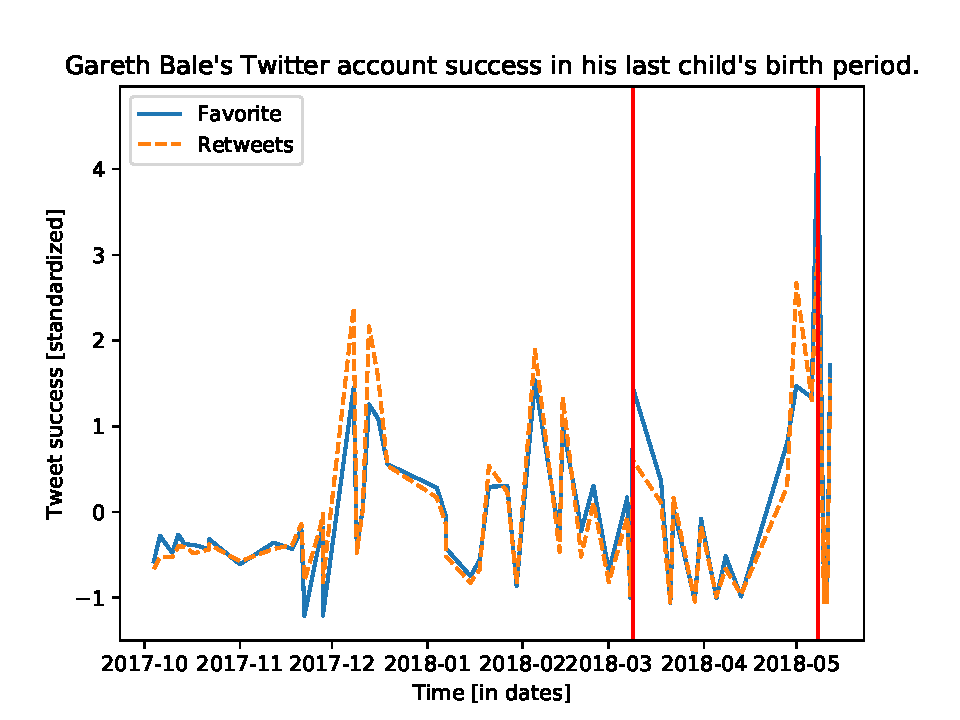
\includegraphics[width=%
0.8\textwidth]{img/bale}
\caption{The success collected by this account is high when it talks about a life event (the two red vertical line represent the publication of two posts related to the birth of a child).}
\label{fig:bale}
\end{figure}

This last function has the goal to analyze the user's timeline to discover a life event in it. Since a life event is something important and rare into a user's life, the assumption is that also in his/her social life his/her behaviour is different when the event is approaching or is in progress. For this reason some unusual patterns, related to the life event itself or to the average success of the posts, are searched for. The idea is that a user does not publishes contents about, for examples, a new baby, very usually, but only when something important is about to happen. In addition to that, a post about a new baby announcement gets probably more feedbacks compared to a normal post, such as congratulation messages \cite{dickinson2015identifying}. The detection of a life event is based on these routine changes, which can be various: a slow but constant increase of interest before the event, or a sudden peak when the event is happening. In general, the relative frequency of activities related to the life event itself is monitored. As shown in figure~\ref{fig:bale}, when the user talks about a life event, the success of his/her post tends to be high.
At this point, a timeline is composed by a list of post, each one with the probability of being about the life event and with the other metadata, like date of publication and post success. Let $p$ be the probability given by the classifier about a post, that post is considered related to the life event if $ p > p_1$. If the previous condition is false, but $p_2 <= p <= p_1 $, the post success is taken into consideration: let $n$ the number of post of a user, and
\[
\mu_\text{likes} = \frac{1}{n} \sum_{i=1}^n p_i.likes \quad \mu_\text{shares} = \frac{1}{n} \sum_{i=1}^n p_i.shares \quad \mu_\text{sentiment} = \frac{1}{n} \sum_{i=1}^n p_i.sentiment
\]
the average of likes, shares and sentiment among all the user's post. If 
\begin{gather}
\label{avgs}
p.likes > \mu_\text{likes} \land p.shares > \mu_\text{shares} \land p.sentiment > \mu_\text{sentiment}
\end{gather}
the post $p$ is considered related to the life event, otherwise no.

For each day $d$ the user has been active on social media (those days in which the user published something), the frequency $f$ is computed as follows:
\begin{gather}
f(d) = \frac{r(d)}{all(d)}
\label{freq}
\end{gather}
where $r(d)$ is the number of posts related to the life event written the day $d$, and $all(d)$ is the count of all posts published the day $d$. Of course, the timeline is already targeted with the life event taken into consideration. In other words, the life event to monitor is chosen in the previous steps: at this point the timeline is labelled only for a single life event. Once the frequency has been computed for every day, it can be plotted over time, and at the moment $f$ passes a given threshold $\alpha$, the life event is begun. When a minimum number of days $\beta$ in which $f(t) > \alpha$ are found, the life event can be considered as detected. By the time in $\gamma$ days there are no \emph{active days}, the life event can be seen as over.

As input is expected a list of boolean label with a timestamp, that represents the user's timeline in function to a life event.

As output, a boolean answer is expected, together with a time range in which the life event has been detected (this range can be composed by the date of the first and the last post related to the life event). Of course, the user may have not lived the life event, so in this case the list will be empty. Also, a person can live a life event more than once, so the output can be a list of labels.

There are several parameter for this phase: 
\begin{itemize}
\item a pair of probability $p_1$ and $p_2$ to consider a post directly related with the life event, or to check post success to take that decision. By default, $p_1 = 0.6$ and $p_2 = 0.4$.
\item the threshold $\alpha$ for the frequency $f$ over which the life event is considered as started.
\item $\beta$, the minimum number of \emph{active posts} to consider a life event detected. This parameter serves to correct any errors in post classification. In fact, is possible that a text or an image is misclassified: using this parameter is possible to avoid single and isolated errors.
\item $\gamma$, the maximum time between two \emph{active days} to consider them as related to the same life event. This parameter has the role to put an end to a detection, and consequently to split two consecutive life events.
\end{itemize}

\section{Interfaces of the components}
\label{sec:apis}
In this section the API of each component will be presented. Internal APIs are very important to allow system scalability and to facilitate any future changes to the logic or to the functionalities. Firstly, some data types used inside the system will be formalized, and secondly, the API will be listed.

The first data type represents a \emph{user}, which is a subject of a computation. The object \texttt{User} is so composed:

\begin{center}
\label{tab:user}
\begin{tabular}{lll}
\hline
User & & \\
\hline
\textbf{Integer} & userID & \%The ID of the user inside the system. It is a unique number \\
\textbf{String} & name & \%The name of the user \\
\textbf{SocialNetworkUser}[] & socials & \%Array of social networks in which she's registered in \\
\hline
\end{tabular}
\end{center}

where a \texttt{SocialNetworkUser} object is so composed:

\begin{center}
\label{tab:social}
\begin{tabular}{lll}
\hline
SocialNetworkUser & & \\
\hline
\textbf{Integer} & socialID & \%The ID of the user inside this specific social network \\
\textbf{String} & name & \%The name of the user in this social network \\
\textbf{Integer} & from & \%ID of the first post downloaded \\
\textbf{Integer} & to & \%ID of the last post downloaded \\
\hline
\end{tabular}
\end{center}

The fields \emph{from} and \emph{to} need to understand where to begin a download request. Finally, the concept of \emph{post} is now formalized in an object call \texttt{Post}: it includes all the useful data for this purpose, such as date of creation, number of likes and shares, sentiment score, entity and topic sets and the probability to be about a life event. At the beginning of the analysis many of this attributes will be empty, and each logical step will add a piece of information. Each post is uniquely identified by the couple (ID, social networks).

\begin{center}
\label{tab:post}
\begin{tabular}{lll}
\hline
Post & & \\
\hline
\textbf{Integer} & postID & \%The ID of the post in the social network\\
\textbf{String} & socialNetwork & \%The social network from where the post comes from \\
\textbf{User} & author & \%The author of the post \\
\textbf{Date} & created & \%The creation date of the post \\
\textbf{Integer} & likes & \%Number of likes received \\
\textbf{Integer} & shares & \%Number of shares \\
\textbf{Float} & sentiment & \%Sentiment score \\
\textbf{Set} & entities & \%Set of strings representing the entities found in post text or images \\
\textbf{Set} & topics & \%Set of strings representing the topics found in post text or images \\
\textbf{Float} & probability & \%Probability of the post to be about a life event \\
\hline
\end{tabular}
\end{center}

Now the API of the four logical component will be presented. Each one can be seen as a web interface that accepts and returns JSON objects. Every time that an object described just above here is used, only the parameters to uniquely identify an instance of these objects will be used. For example, only a \texttt{userID} will be used to indicate an \texttt{User} instance.

\subsection{Collector API}
The collector needs a \texttt{User} instance to which fetch her contents online, and a count that indicates how many activities to download from each social network.

Input:
\begin{itemize}
\item \texttt{userID}, Integer.
\item \texttt{count}, Integer.
\end{itemize}

Output:
\begin{itemize}
\item a list of \texttt{Post} identified by \texttt{postID} and \texttt{socialNetwork}.
\end{itemize}

Below an example of input and output.

\begin{Verbatim}
//input
{
	"userID": 2565227499,
	"count": 200
}

//output
[
	{
		"postID": 667069250268479488,
		"socialNetwork": "Twitter"
	}
]
\end{Verbatim}

\subsection{Entity extraction API}
The extractor needs a \texttt{Post} instance to which extract entities, and returns the same instance enriched.

Input and output are the same:
\begin{itemize}
\item \texttt{postID}, Integer.
\item \texttt{socialNetwork}, String.
\end{itemize}

Below an example in JSON format. Both input and output are the same.

\begin{Verbatim}
{
	"postID": 667069250268479488,
	"socialNetwork": "Twitter"
}
\end{Verbatim}

\subsection{Classifier API}
The classifier takes a life event on which the classification will be done, and a list of \texttt{Post} instances and adds the attributes \texttt{probability}, that indicates the probability with which each post is about the life event. It returns the same instances with the probability added.

Input:
\begin{itemize}
\item \texttt{lifeEvent}, String.
\item a list of \texttt{Post}, each one identified by \texttt{postID} and \texttt{socialNetwork}.
\end{itemize}

Output:
\begin{itemize}
\item a list of \texttt{Post}, each one identified by \texttt{postID} and \texttt{socialNetwork}.
\end{itemize}

Below an example of input and output.

\begin{Verbatim}
//input
{
	"lifeEvent": "Having children",
	"posts": [
		{
			"postID": 667069250268479488,
			"socialNetwork": "Twitter"
		}
	]
}

//output
[
	{
		"postID": 667069250268479488,
		"socialNetwork": "Twitter"
	}
]
\end{Verbatim}

\subsection{Computator API}
The computator needs a list of \texttt{Post}, which represents the user's \emph{timeline}. Each one has to have a probability of being about a life event. It returns a list of pairs of dates, each one indicating the beginning and the end of a life event found in the timeline. The list can be empty.

Input:
\begin{itemize}
\item a list of \texttt{Post}, each one identified by \texttt{postID} and \texttt{socialNetwork}.
\end{itemize}

Output:
\begin{itemize}
\item a list of pairs of dates.
\end{itemize}

An example of input and output is presented below.

\begin{Verbatim}
//input
[
	{
		"postID": 667069250268479488,
		"socialNetwork": "Twitter"
	}
]

//output
[
	{
		"from": "2018-3-8",
		"to": "2018-5-24"
	}
]
\end{Verbatim}

\section{The detection algorithm}
\label{sec:alg}

In this subsection the detection algorithm, whose logic was previously explained in section~\ref{sec:computationperformer}, will be defined in pseudocode. It is assumed that all the parameters previously highlighted are defined, and that all the tree previous logical steps are already been executed. Let $n$ be the number of posts in the timeline taken into analysis, and let the data type \texttt{Post} defined as in~\ref{tab:post}.

The algorithm is composed by two main parts. In the first part, the goal is to compute the average number of likes and shares received by the user among her posts, and the average sentiment score. After that, all the posts are grouped by date of publication, creating a dictionary with keys $k$ the days in which the user has published something, and values a tuple (posts related with the life event on day $k$, all posts on day $k$). This is explain in the algorithm~\ref{freq_computing}.

\begin{algorithm}
\caption{Compute the relative frequency of activities related to the life event.}
\label{freq_computing}
\begin{algorithmic}[1]
\Require posts must be sorted by date
\Function{computeFrequency}{Post[] posts}
\State $AVGLikes \gets \frac{1}{n} \sum_{i=1}^n p_i.likes $
\State $AVGShares \gets \frac{1}{n} \sum_{i=1}^n p_i.shares $
\State $AVGSentiment \gets \frac{1}{n} \sum_{i=1}^n p_i.sentiment$
\State $frequencies \gets \{\}$
\State $count \gets 0$
\State $total \gets 0$
\For{$i \gets 1 \text{ to } n$}
	\State $total \gets total + 1$
	\If{$posts[i].probability > p_1$}
		\State $count \gets count + 1$
	\ElsIf{$posts[i].probability \geq p_2 \land posts[i].likes > AVGLikes \land posts[i].shares > AVGShares \land posts[i].sentiment > AVGSentiment$}
		\State $count \gets count + 1$
	\EndIf
	\If{$i = n \lor posts[i].created \ne posts[i + 1].created$}
		\State $frequencies[posts[i].created] \gets (count, total)$
	\EndIf
\EndFor
\Return $frequencies$
\EndFunction 
\end{algorithmic}
\end{algorithm}

For each day $count$ and $total$ are computed, which represent the number of posts related to the life event and the total number of post on that day respectively. At line 10 the decision to trust the classification directly is taken. In case it's not trusted, the condition at line 12 checks whether the probability is greater or equal than $p_2$ and if number of likes, shares and sentiment score are all over the average of the user, as explained in formula~\ref{avgs}. The last condition at line 14 is to understand whether a post is the last one for a day: this happens when the current post is the last one in the collection, or when the next one has a different date of creation.

In the second part the dictionary with counters is analyzed, computing for each day the frequency of activeness as in formula~\ref{freq} and analyzing it to understand if there are significant changes on it. This is explained in the algorithm~\ref{decision}.

\begin{algorithm}
\caption{Decide whether a user has lived a life event}
\label{decision}
\begin{algorithmic}[1]
\Function{DetectLifeEvents}{frequencies}
\State $start \gets today()$
\State $end \gets \perp$
\State $count \gets 0$
\State $found \gets \{\}$
\ForAll{$k \in \text{frequencies}$}
	\State $f \gets \frac{\text{frequencies}[k].count}{\text{frequencies}[k].total}$
	\If{$f > \alpha$}
		\If{$k < start$}
			\State $start \gets k$
			\State $end \gets k$
		\EndIf
		\If{$(k - end) < \gamma$}
			\State $end \gets k$
			\State $count \gets \text{frequencies}[k].count$
		\Else
			\If{$count \geq \beta$}
				\State $found \gets found \cup \{(start, end)\}$
			\EndIf
			\State $start \gets k$
			\State $end \gets k$
			\State $count \gets 1$
		\EndIf
	\EndIf
\EndFor
\If{$count \geq \beta \land end \ne \perp$}
	\State $found \gets found \cup \{(start, end)\}$
\EndIf
\Return $found$
\EndFunction
\end{algorithmic}
\end{algorithm}

The symbol $\perp$ represents a null type. The idea is to find some time intervals that represent a life event, each one recognized by a $start$ and an $end$. For each day in which the user published something, the relative frequency $f$ is computed (at line 7) as shown in formula~\ref{freq}. If $f$ is greater than the threshold $\alpha$ and is the very first day encountered, $start$ will point to it. For every other following day in which $f > \alpha$ and that is less than $\gamma$ days later than the current $end$, $end$ is overwritten, to point to that day. When an active day is too far from the last active day, the conditions to add a life event are checked (line 16): if at least $\beta$ active posts were previously found, the life event from $start$ to $end$ is added, and these variables are restored to detect another interval. In the end, at line 21, is verified whether there is an interval left open, and in this case, if there are enough posts, a last life event is added.

The complexity of both algorithm~\ref{freq_computing} and~\ref{decision} is $\Theta(n)$ in time, because each post is analyzed only once, in both functions. In case posts are not sorted by date, the computational cost will be dominated by the sorting procedure, becoming $\Theta(n \log n)$.

\section{Exposed APIs}
\label{sec:APIs}

In this section the APIs offered by the system will be defined. These interfaces are RESTful APIs, which expose the main resources available in the system: \texttt{User}, \texttt{Download Request} and \texttt{Computation}. For each resource, the possibilities to retrieve and create new instances are offered, and for the user resource is also possible to edit an instance. The structure of the \texttt{User} resource is described in section~\ref{sec:apis}. A \texttt{Download Request} is meant to download user's contents from social media, and it's executed asynchronously, as explained in section~\ref{sec:downloadqueues}. Finally, a \texttt{Computation} is an analysis on a user's timeline with a given life event, as described in section~\ref{sec:alg}.

Each response has a field \texttt{"ok"} that indicates whether everything went well. In case an error occurs, the field \texttt{"error"} will give a human readable explanation of the error, while the HTTP status code will indicate what kind of problem occurred (for example a 404 error in case the user requires a resources that doesn't exist).

The complete API specification can be found on Apiary\footnote{\url{apiary.io}}:
\begin{center}
\url{lifeevents.docs.apiary.io}
\end{center}


      \chapter{Results}
\label{cha:results}
In this chapter will be illustrated the results obtained in the various texts carried out on the system. Firstly, the performance of the classifier will be explained, and secondly \dots

\section{Classification performance}
The first method experimented to implement the classifier was a data driven approach. 

The dataset taken from \cite{dickinson2015identifying} was filtered, keeping only tweets about a wedding or a birth of a child. Then it was splitted in two files, one for each life event, and every tweet was enriched with Wikipedia entities and topics using the external semantic analyzer. In the end, the wedding dataset counted $2538$ samples, the births one $2233$. According to the literature, a naive bayes classifier and a decision tree were chosen as classifiers, but due to the better performance of the first one, the second one was discarded. In particular, the classifier was a Multinomial Naive Bayes\footnote{\url{http://scikit-learn.org/stable/modules/naive_bayes.html#multinomial-naive-bayes}} available in the \texttt{scikit-learn}\footnote{\url{http://scikit-learn.org/}} library \cite{scikit-learn}.

The very first feature extraction technique was inspired by the \texttt{tf-idf} weight function\footnote{\url{https://it.wikipedia.org/wiki/Tf-idf}}, which is used to undestrand the importance of a word into a series of documents. The idea was to select a small sample of key entities analyzing some web pages focused on the life event taken into consideration, such as a wedding planner homepage or a pregnancy blog. These $k$ top entities were used as features of tweets, and a matrix $X$ was created, with a number of rows equals to the number of tweets and $k$ columns. Each element [$i,j$] of $X$ was a counter of how many times the entity (or topic) $j$ was found in the tweet $i$. However, this methodology performed worse than a random classifier, with both precision and recall scores lower than $0.5$, with $k = 3, 4, 5, 10, 100$.

\begin{table}
\begin{center}
\begin{tabular}{cccc}
\hline
Life event & Precision & Recall & F1 Score \\
\hline
\textbf{Getting married} & $0.82$ & $0.81$ & $0.81$ \\
\textbf{Having children} & $0.77$ & $0.78$ & $0.77$ \\
\hline
\end{tabular}
\end{center}
\caption{The performance of the first classifier on a single dataset split.}
\label{tab:singlesplit}
\end{table}

\begin{table}
\begin{center}
\begin{tabular}{cccc}
\hline
Life event & Precision & Recall & F1 Score \\
\hline
\textbf{Getting married} & $0.73$ & $0.82$ & $0.77$ \\
\textbf{Having children} & $0.62$ & $0.57$ & $0.59$ \\
\hline
\end{tabular}
\end{center}
\caption{The performance of the first classifier on a 10 fold cross validation.}
\label{tab:kfold}
\end{table}

A much better performance with the dataset, but unfortunately not with the reality, was given by using all the Wikipedia entities of the training set as features. Firstly, the dataset was splitted into a training and a test set, the first one with the 70\% of the samples and the second with the remaining 30\%; secondly, a matrix $X$ was created in the same way of the previous attempt, with the difference that this time the number of columns was in the order of thousands. On the test set this solution had good results, as shown in tables~\ref{tab:singlesplit} and \ref{tab:kfold}, but in the reality, trying to predict if tweets from a user timeline were about or not a life event, this solution turned out to be impractical: the discrimination was too loose, and many tweets that wasn't related with the life event at all were considered "positives", with the precision measure that fell dramatically under $0.1$. The overfitting reason was excluded, because the training set was kept aside from everything else. In addition, each sample in the dataset was written by a unique user. The most probable reason is that the dataset used for the training was too balanced compared to the real situation in social networks: in fact, while the dataset contains about 50\% of tweets about a life event and 50\% not, a timeline has a very small percentage of contents about a life event. For example, analyzing a portion of Gareth Bale's Twitter profile\footnote{\url{https://twitter.com/GarethBale11}}, it turned out that on 224 tweets only 2 were about the birth of a child and only one about marriage. Many other profiles considered had similar proportions. 

A third approach was tried, with the purpose of improve the previous situation: train the classifier with a very unbalanced dataset, discarding randomly many of the positive samples to create a 90\% negatives and 10\% positives situation. In each test the positive subset were different, because of randomness, but as before the results were good only with the test set: with a real profile the discrimination was too strong this time, not finding any tweet at all, maybe just because of this disproportion, where too few related samples were given and so the classifier didn't see enough entities among those of positive samples.

The biggest problem at all was caused by the external semantic analyzer - Dandelion - used to discover Wikipedia entities inside texts. Its results turned out to be very inaccurate for such short texts written in Twitter: for example, a tweet published by a famous sports man about his wedding, with the text "\textit{This is her, my wife}"\footnote{\url{https://twitter.com/petosagan/status/667069250268479488}} was mapped by the analyzer to a song by the British rock band \textit{the Who} called \textit{My Wife}, not undestanding the context at all. Some other cases of misunderstanding between the text and its true meaning were found, for example the word \textit{congratulations} was mapped into the entity "\texttt{Congratulations: 50 Years of the Eurovision Song Contest}", but this was not a big issue because this combination was always respected every time that word was found. Just to be sure that some words were recognized correctly, 4 keywords for each event were manually mapped into their correct entities, such as \textit{baby} on the entity \texttt{Infant}.

\begin{figure}
\centering
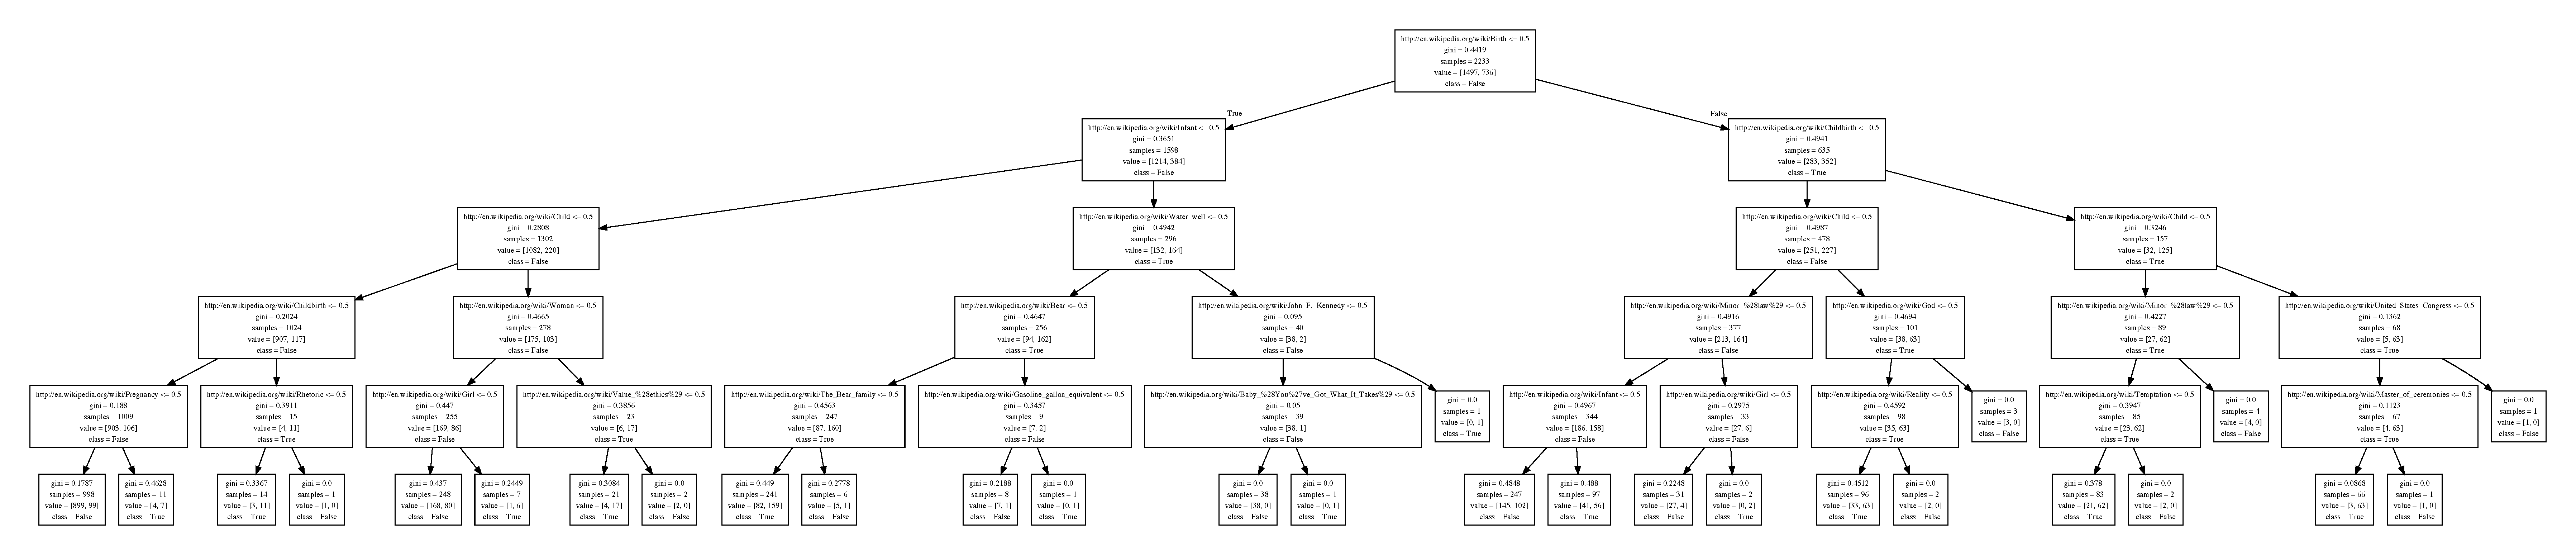
\includegraphics[width=%
0.95\textwidth]{img/decisiontree}
\caption{The decision tree for the birth of a child event. As can be seen, the nearest nodes to the root are decisions about entities that are strickly connected with the life event itself, and each of them makes a significant split in terms of the size of the resulting subsets, while the most deep nodes are strongly connected with the training set. For this reason the maximum depth was forced to be low.}
\label{fig:decisiontree}
\end{figure}

To avoid issues with the semantic analyzer as much as possible, as few as possible entities were used to classify a tweet: a very first approach consisted in a manual selection of features, for example the entity \texttt{Wife} for wedding, but the results were not satisfactory. The ultimate approach was to let the data decide which entities to use, relying on the dataset taken from \cite{dickinson2015identifying}. The classifier was changed, opting for a decision tree. A decision tree is a machine learning model used for regression and classification based on a binary tree data structure. Each node of the tree is a question relative to a feature of the objects to classifiy, and each leaf represent a decision, an estimation of the value of the input object. During the training, the tree is build starting from the root: at each step of the construction, the goal is to split the dataset into two, making a question on a feature of the objects, to reduce the unpredictability of the two new subsets as much as possible. Every object in input will have its path from the root to a single leaf, which will represent the decision. Precisely, the classifier was the decision tree offered by the \texttt{scikit-learn} library\footnote{\url{http://scikit-learn.org/stable/modules/generated/sklearn.tree.DecisionTreeClassifier.html}}. To reduce the overfitting on the training data, the maximum depth of the tree was limited to 5, so for each root-leaf path, at most 4 intermediate nodes could be found. The decision tree for the life event \texttt{Having Children} can be seen in figure~\ref{fig:decisiontree}. The results with the dataset of \cite{dickinson2015identifying} were a little worse than those of the bayesian classifier shown in tables~\ref{tab:singlesplit} and \ref{tab:kfold}, but in the reality, with a test conducted on 5836 tweets taken by 43 different timelines the results were much better than the previous one, as explained in tables~\ref{tab:treewedding} and \ref{tab:treechild}.

\begin{table}[htbp]
\centering
\subtable[Results about wedding tweets\label{tab:treewedding}]{%
\begin{tabular}{ccccc}
\hline
Sample & Precision & Recall & F1 Score & Support \\
\hline
\textbf{True} & $0.87$ & $0.70$ & $0.77$ & $134$ \\
\textbf{False} & $0.91$ & $0.97$ & $0.94$ & $5702$ \\
\textbf{Avg / Total} & $0.90$ & $0.90$ & $0.90$ & $5836$ \\
\hline
\end{tabular}
}\qquad\qquad
\subtable[Results about birth of a child tweets\label{tab:treechild}]{%
\begin{tabular}{ccccc}
\hline
Sample & Precision & Recall & F1 Score & Support \\
\hline
\textbf{True} & $0.65$ & $0.62$ & $0.63$ & $161$ \\
\textbf{False} & $0.93$ & $0.94$ & $0.94$ & $5675$ \\
\textbf{Avg / Total} & $0.89$ & $0.89$ & $0.89$ & $5836$ \\
\hline
\end{tabular}
}
\caption{The performance of the decision tree with tweets from a small set of authors. The previous classifier, the naive bayes, showed both precision and recall scores under 0.1.}
\end{table}
      \chapter{Conclusions}
\label{cha:conclusions}
This thesis answers the research question about the feasibility of life event detection on social media, presenting a solution to detect two types of life events into social network timelines. It goes beyond the actual state of the art, because it's not limited to a post classification only, but it does a social profile analysis to discover an event. Furthermore, it uses a technique based on Wikipedia contents to understand what the user talkes about, which gives to the system an high scalability, allowing the adding of a new language to support in a more easily way than a traditional language undestranding system. In addition to that, it's possible to consider all the components of a post (text, images, external links, etc.) as \emph{entity containers}, permitting an easier training in terms of quantity and type of data: in fact in this way it's not necessary to have one training set for texts and one for photos, but just a set of \emph{posts} about life events, each of them can be made by texts only, picture only or both.

The classifier showed some very good results, with both \emph{precision} and \emph{recall} measures around $0.9$, and the whole detection system had encouraging results with ample room for improvement, considering that due to GDPR issues and to the resulting new policies of social media only textual contents from Twitter were used for tests.

In addition to that, a new dataset about life event posts on Twitter were release, containing 5836 samples composed by 45 users, 161 about weddings and 134 about births of a child. It was created deliberately so unbalance because it has the purpose to simulate how is someone's timeline on social networks, where these kinds of posts are very rare by and large. This dataset is freely available and usable, and can be found here:
\begin{center}
\url{doi.org/10.5281/zenodo.1294893}
\end{center}

\section{Future work}
\label{sec:futurework}
There are several aspects that can be deepened or added. First of all, this system was projected to work with several social networks, but due to the reasons explained in section~\ref{sec:choices} only Twitter and textual contents were taken into consideration during the development phase. So the first possible addition can be adding the support for \emph{Facebook} and \emph{Instagram}, and also analyze images for post classification. Furthermore, this latters social media are more used than Twitter to share personal contents and news, such as the own marriage or the birth of a child, and many posts about life events are full of images, or even composed by images only.

A possible way to make results better could be the analysis of the comments of a post: a post about a life event is usually full of comments of congratulations, nearness and support. Comments can give a better view of the context of the post, and so they can lead to a better understanding.

Another future expansion could be the addition of other life events, like graduation, buying a new home, changing a job, the death of somebody, etc. Each of them has its own meaning and brings with it a series of consequences or necessities.

In addition to that, it's possible to combine the result coming from the detection algorithm with some demographic studies or some statistical data, to refine the results. In this way it would be possible to weight the information coming from social medias with external data, provided by some statistical institute or other trusted sources.

Another possibility could be expand the machine learning capability of the system: in addition to the already current event detection, also predict a life event would give such a powerful piece of information.

In conclusion, this thesis work offers a good base for detecting life events on social networks, which can be boosted or deepened in some aspects, for example, based on the scope in which it will be used, or on what type of users it will work mainly. Any addiction will still follow a logic or patterns very similar to those explained in this dissertion.
      
    \endgroup


    % bibliografia in formato bibtex
    %
    % aggiunta del capitolo nell'indice
    \addcontentsline{toc}{chapter}{Bibliography}
    % stile con ordinamento alfabetico in funzione degli autori
    \bibliographystyle{plain}
    \bibliography{biblio}
%%%%%%%%%%%%%%%%%%%%%%%%%%%%%%%%%%%%%%%%%%%%%%%%%%%%%%%%%%%%%%%%%%%%%%%%%%
%%%%%%%%%%%%%%%%%%%%%%%%%%%%%%%%%%%%%%%%%%%%%%%%%%%%%%%%%%%%%%%%%%%%%%%%%%
%% Nota
%%%%%%%%%%%%%%%%%%%%%%%%%%%%%%%%%%%%%%%%%%%%%%%%%%%%%%%%%%%%%%%%%%%%%%%%%%
%% Nella bibliografia devono essere riportati tutte le fonti consultate 
%% per lo svolgimento della tesi. La bibliografia deve essere redatta 
%% in ordine alfabetico sul cognome del primo autore. 
%% 
%% La forma della citazione bibliografica va inserita secondo la fonte utilizzata:
%% 
%% LIBRI
%% Cognome e iniziale del nome autore/autori, la data di edizione, titolo, casa editrice, eventuale numero dell’edizione. 
%% 
%% ARTICOLI DI RIVISTA
%% Cognome e iniziale del nome autore/autori, titolo articolo, titolo rivista, volume, numero, numero di pagine.
%% 
%% ARTICOLI DI CONFERENZA
%% Cognome e iniziale del nome autore/autori (anno), titolo articolo, titolo conferenza, luogo della conferenza (città e paese), date della conferenza, numero di pagine. 
%% 
%% SITOGRAFIA
%% La sitografia contiene un elenco di indirizzi Web consultati e disposti in ordine alfabetico. 
%% E’ necessario:
%%   Copiare la URL (l’indirizzo web) specifica della pagina consultata
%%   Se disponibile, indicare il cognome e nome dell’autore, il titolo ed eventuale sottotitolo del testo
%%   Se disponibile, inserire la data di ultima consultazione della risorsa (gg/mm/aaaa).    
%%%%%%%%%%%%%%%%%%%%%%%%%%%%%%%%%%%%%%%%%%%%%%%%%%%%%%%%%%%%%%%%%%%%%%%%%%
%%%%%%%%%%%%%%%%%%%%%%%%%%%%%%%%%%%%%%%%%%%%%%%%%%%%%%%%%%%%%%%%%%%%%%%%%%
    

%    \titleformat{\chapter}
%        {\normalfont\Huge\bfseries}{Allegato \thechapter}{1em}{}
    % sezione Allegati - opzionale
%    \appendix
%    \chapter{Titolo primo allegato}

Lorem ipsum dolor sit amet, consectetur adipiscing elit. Donec sed nunc orci. Aliquam nec nisl vitae sapien pulvinar dictum quis non urna. Suspendisse at dui a erat aliquam vestibulum. Quisque ultrices pellentesque pellentesque. Pellentesque egestas quam sed blandit tempus. Sed congue nec risus posuere euismod. Maecenas ut lacus id mauris sagittis egestas a eu dui. Class aptent taciti sociosqu ad litora torquent per conubia nostra, per inceptos himenaeos. Pellentesque at ultrices tellus. Ut eu purus eget sem iaculis ultricies sed non lorem. Curabitur gravida dui eget ex vestibulum venenatis. Phasellus gravida tellus velit, non eleifend justo lobortis eget. 

\section{Titolo}
Lorem ipsum dolor sit amet, consectetur adipiscing elit. Donec sed nunc orci. Aliquam nec nisl vitae sapien pulvinar dictum quis non urna. Suspendisse at dui a erat aliquam vestibulum. Quisque ultrices pellentesque pellentesque. Pellentesque egestas quam sed blandit tempus. Sed congue nec risus posuere euismod. Maecenas ut lacus id mauris sagittis egestas a eu dui. Class aptent taciti sociosqu ad litora torquent per conubia nostra, per inceptos himenaeos. Pellentesque at ultrices tellus. Ut eu purus eget sem iaculis ultricies sed non lorem. Curabitur gravida dui eget ex vestibulum venenatis. Phasellus gravida tellus velit, non eleifend justo lobortis eget. 

\subsection{Sottotitolo}
Lorem ipsum dolor sit amet, consectetur adipiscing elit. Donec sed nunc orci. Aliquam nec nisl vitae sapien pulvinar dictum quis non urna. Suspendisse at dui a erat aliquam vestibulum. Quisque ultrices pellentesque pellentesque. Pellentesque egestas quam sed blandit tempus. Sed congue nec risus posuere euismod. Maecenas ut lacus id mauris sagittis egestas a eu dui. Class aptent taciti sociosqu ad litora torquent per conubia nostra, per inceptos himenaeos. Pellentesque at ultrices tellus. Ut eu purus eget sem iaculis ultricies sed non lorem. Curabitur gravida dui eget ex vestibulum venenatis. Phasellus gravida tellus velit, non eleifend justo lobortis eget. 


\chapter{Titolo secondo allegato}

Lorem ipsum dolor sit amet, consectetur adipiscing elit. Donec sed nunc orci. Aliquam nec nisl vitae sapien pulvinar dictum quis non urna. Suspendisse at dui a erat aliquam vestibulum. Quisque ultrices pellentesque pellentesque. Pellentesque egestas quam sed blandit tempus. Sed congue nec risus posuere euismod. Maecenas ut lacus id mauris sagittis egestas a eu dui. Class aptent taciti sociosqu ad litora torquent per conubia nostra, per inceptos himenaeos. Pellentesque at ultrices tellus. Ut eu purus eget sem iaculis ultricies sed non lorem. Curabitur gravida dui eget ex vestibulum venenatis. Phasellus gravida tellus velit, non eleifend justo lobortis eget. 

\section{Titolo}
Lorem ipsum dolor sit amet, consectetur adipiscing elit. Donec sed nunc orci. Aliquam nec nisl vitae sapien pulvinar dictum quis non urna. Suspendisse at dui a erat aliquam vestibulum. Quisque ultrices pellentesque pellentesque. Pellentesque egestas quam sed blandit tempus. Sed congue nec risus posuere euismod. Maecenas ut lacus id mauris sagittis egestas a eu dui. Class aptent taciti sociosqu ad litora torquent per conubia nostra, per inceptos himenaeos. Pellentesque at ultrices tellus. Ut eu purus eget sem iaculis ultricies sed non lorem. Curabitur gravida dui eget ex vestibulum venenatis. Phasellus gravida tellus velit, non eleifend justo lobortis eget. 

\subsection{Sottotitolo}
Lorem ipsum dolor sit amet, consectetur adipiscing elit. Donec sed nunc orci. Aliquam nec nisl vitae sapien pulvinar dictum quis non urna. Suspendisse at dui a erat aliquam vestibulum. Quisque ultrices pellentesque pellentesque. Pellentesque egestas quam sed blandit tempus. Sed congue nec risus posuere euismod. Maecenas ut lacus id mauris sagittis egestas a eu dui. Class aptent taciti sociosqu ad litora torquent per conubia nostra, per inceptos himenaeos. Pellentesque at ultrices tellus. Ut eu purus eget sem iaculis ultricies sed non lorem. Curabitur gravida dui eget ex vestibulum venenatis. Phasellus gravida tellus velit, non eleifend justo lobortis eget. 




\end{document}
